\documentclass[11pt, twoside, a4paper]{article}

\usepackage[top=15mm, bottom=15mm, left=25mm, right=25mm]{geometry}
\usepackage{tikz}
\usepackage{amssymb,amsmath, amsthm}
\usepackage[labelsep=period]{caption}

\newtheorem{theorem}{Theorem}[section]
\newtheorem{corollary}{Corollary}[theorem]
\newtheorem{lemma}[theorem]{Lemma}

\theoremstyle{definition}
\newtheorem{definition}{Definition}[section]

\newcommand{\Fig}[1]{Figure~\ref{fig:#1}}
\newcommand{\Eq}[1]{Eq.~(\ref{eq:#1})}
\newcommand{\Eqs}[2]{Eqs.~(\ref{eq:#1})--(\ref{eq:#2})}
\newcommand{\set}[1]{\mathbb{#1}}
\newcommand{\Th}[1]{Theorem~\ref{th:#1}}
\newcommand{\Le}[1]{Lemma~\ref{le:#1}}

\newcommand{\xpm}{\ensuremath{x_\pm}}
\newcommand{\xmp}{\ensuremath{x_\mp}}
\newcommand{\ypm}{\ensuremath{y_\pm}}
\newcommand{\ymp}{\ensuremath{y_\mp}}
    
\newcommand{\inv}[1]{#1^{-1}}

\begin{document}
\title{Euler 94: Almost equilateral triangles}
\date{}
\author{Didier Pieroux}
\maketitle

%===============================================================================
\begin{abstract} 

It is easily proved that no equilateral triangle exists with integral length sides and integral area. However, the almost equilateral triangle 5-5-6 has an area of 12 square units. We shall define an almost equilateral triangle to be a triangle for which two sides are equal and the third differs by no more than one unit. Find the sum of the perimeters of all almost equilateral triangles with integral side lengths and area and whose perimeters do not exceed one billion (1,000,000,000).
\end{abstract}

%===============================================================================
\section{Formulation}

We have to find all isosceles triangles whose base $b\in\set N$ and equal sides $c \in\set N$ differ by one. Let's label $h$ the height of such a triangle (\Fig{triangle1}).
\begin{figure}[h]
    \begin{center}
        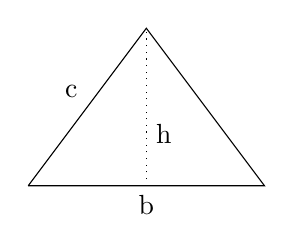
\begin{tikzpicture}[scale=0.5]
        \draw (0, 0) 
           -- (6, 0) node[midway, below] {b} 
           -- (3, 4) 
           -- (0, 0) node[midway, above left] {c} ;
        \draw[dotted] (3, 0) -- (3, 4) node[pos=0.33, right] {h};
        \end{tikzpicture}
        \caption{Illustration of the Labels used.}
        \label{fig:triangle1}
    \end{center}
\end{figure}

The problem is then described by the following equations, with $P$ the perimeter and $S$ the area:
\begin{align}
    c^2 & = (b/2)^2 + h^2 \label{eq:pytha1} \\ 
    c & = b \pm 1 \label{eq:ab} \\ 
    P & = 2c+b \\ 
    S & = h b/2 \text{ with } S \in\set N \label{eq:S1}
\end{align} 
    
\begin{lemma}$b$ is even.\end{lemma}
\begin{proof} Suppose $b$ odd. \Eq{S1} implies that $h$ must be even and integer for $S$ to be integral. But then $c^2 = b^2/4 + h^2$ is not integral, which is impossible as $c$ is integral.
\end{proof}

For ease, let us pose $b=2a$ with $a\in\set N$ (\Fig{triangle2}). 
\begin{figure}
    \begin{center}
        \begin{tikzpicture}[scale=0.5]
        \draw          (0, 0) -- (3, 0) node[midway, below] {a};
        \draw [dashed] (3, 0) -- (6, 0) -- (3, 4);
        \draw          (3, 4) -- (0, 0) node[midway, above left] {c} ;
        \draw [dotted] (3, 0) -- (3, 4) node[pos=0.33, right] {h};
        \end{tikzpicture}
        \caption{Illustration of the Labels used (reduced problem).}
        \label{fig:triangle2}
    \end{center}
\end{figure}

The \Eqs{pytha1}{S1} read now:
\begin{eqnarray}
c^2 & = & a^2 + h^2  \label{eq:pytha2} \\
  c & = & 2a \pm 1  \label{eq:ac} \\
  P & = & 2(a+c) \\ 
  S & = & ah \label{eq:S2}
\end{eqnarray}

The triple $(a, h, c)$ is thus Pythagorean\footnote{https://en.wikipedia.org/wiki/Pythagorean\_triple}.

\begin{lemma}
	$a$, $h$ and $c$ are pair-wise coprime. 
\end{lemma}

\begin{proof} 
	Suppose that $a$ and $c$ have a common factor $\lambda\in\set N$: $a=\lambda a'$ and $c=\lambda c'$. From \Eq{ac}, it comes $c' = 2 a' \pm 1/\lambda$, which would imply that $c'$ is not integral.
	
	Suppose now that $c$ and $h$ have a common factor. \Eq{pytha2} implies that it must be a factor of $a$; therefore $c$ and $a$ would not be coprime. Similarly if $a$ and $h$ have a common factor, \Eq{pytha2} implies that it must be a factor of $c$; therefore $c$ and $a$ would not be coprime.
\end{proof}

As a consequence valid triple $(a, h, c)$ are primitive Pythagorean triple (PPT).

\section{Tree of primitive Pythagorean triples}
Let the infinitely-deep ternary tree whose root is the Pythagorean triple $p=(3, 4, 5)$ and whose internal nodes are the left-multiplication of their parent node, interpreted as a column vector, by one of the following matrices:
		\[
		A = \left(\begin{matrix}  1 & -2 & 2 \\  2 & -1 & 2 \\  2 & -2 & 3 \end{matrix} \right)\!,\ 
		B = \left(\begin{matrix}  1 &  2 & 2 \\  2 &  1 & 2 \\  2 &  2 & 3 \end{matrix} \right)\!\text{ and }
		C = \left(\begin{matrix} -1 &  2 & 2 \\ -2 &  1 & 2 \\ -2 &  2 & 3 \end{matrix} \right)\!.
		\]
Otherwise said, the nodes of the tree are, in breadth-first order:
\[p, Ap, Bp, Cp, A\!Ap, B\!Ap, C\!Ap, A\!Bp, B\!Bp, C\!Bp, \ldots\] 

\begin{theorem}\label{th:tree}
It can be shown that all the PPTs, and only them, are generated without duplication by this tree\footnote{For a proof see https://en.wikipedia.org/wiki/Tree\_of\_primitive\_Pythagorean\_triples}.
\end{theorem}
    
Because of \Eq{ac}, we are only interested in PPTs of the form $\xmp\!=\!(x, y, 2x\!\pm\!1)$ and $\ypm\!=\!(x, y, 2y\!\pm\!1)$.
\begin{lemma}
The product of $A$ with a PPT \ypm\ produces a PPT \xmp. Similarly, the product of $C$ with a PPT \xpm\ produces a PPT \ymp.
\end{lemma}
\begin{proof}
By \Th{tree}, the product of a PPT by $A$ or $B$ is also a PPT. Calculating explicitly $A \ypm$ shows that the result has the form \xmp. Idem for $B \xpm$ which produces a \ymp.
\end{proof}

\begin{lemma}\label{le:inverse}
Given a PPT $\pi\!=\!(x, y, z)$, 
\begin{itemize}
\item $\inv A\pi$ is a PPT iff $4x<3y$;
\item $\inv B\pi$ is a PPT iff $3x<4y \text{ and } 3y<4x$;
\item $\inv C\pi$ is a PPT iff $4y<3x$.
\end{itemize}
\end{lemma}
\begin{proof}
By carrying out the calculation, it is easily shown that
\begin{itemize}
    \item the Pythagorean relation $x^2+y^2=z^2$ is preserved by multiplication of the inverse matrices, 
    \item the components of the result are positive iff the inequalities of the lemme are fulfilled.
\end{itemize}
We still have to show that the result is primitive. If it wasn't, the components of $\inv A\pi$ would have a common factor. But then the components of $A\inv A\pi=\pi$ would also have that common factor, which is forbidden as $\pi$ is primitive.
\end{proof}

\begin{lemma}
Assuming the inequalities of \Le{inverse}, the product of $\inv A$ with a PPT of the form \xpm\ gives a PPT of the form \ymp. Similarly, the product of $\inv C$ with a PPT of the form \ypm\ gives a PPT of the form \xmp.
\end{lemma}
\begin{proof}
From \Le{inverse}, the result is a PPT. The relations between the components are verified through explicit calculation.
\end{proof}

\begin{lemma}\label{le:predecessor1}
Excepted for $(3, 4, 5)$ which has no predecessor, all PPTs of the form \xpm\ have a predecessor of the form \ymp.
\end{lemma}
\begin{proof}
Since \xpm\ is a PPT different of $(3, 4, 5)$, \Th{tree} implies that it has a parent node. If that parent is not of the form \ymp, then \xpm\ is not generated from it by the matrix $A$, but by the matrix $B$ or $C$. Then (\Le{inverse}) implies that $3y<4x$. As \xpm\ fulfils the Pythagorean equality, it comes $x^2+y^2=z^2=4x^2\pm4x+1$, or $y^2=3x^2\pm4x+1$. $3y<4x$ then implies that $11x^2\pm36x+9<0$. This inequality can be verified only for the $-$ sign and if $3/11<x<3$. But this asks for $x=1$ or $x=2$, for which there is no PPT. This contradiction implies that the parent node must be of the from \ymp.
\end{proof}

\begin{lemma}\label{le:predecessor2}
All PPTs of the form \ypm\ have a predecessor of the form \xmp.
\end{lemma}
\begin{proof}The demonstration is similar to the previous one.\end{proof}

\begin{theorem}\label{th:PPT_branch}
Starting from $(3,4,5)$, multiplying it by C, then multiplying the result by A, then multiplying again that result by C\ldots generates all the PPTs satisfying \Eq{ac}.
\end{theorem}
\begin{proof}
Excepted for $(3, 4, 5)$ which has no predecessor, Lemmas~\ref{le:predecessor1} and \ref{le:predecessor2} show that any other PPT satisfying \Eq{ac} must have a predecessor also satisfying \Eq{ac}. Therefore, starting from any of such a PPT and going from predecessor to predecessor, we move towards the root of the PPT tree, until $(3, 4, 5)$ is finally reached.
\end{proof}

\section{Iterative process}
\subsection{Reduction to a unique transformation}
As seen above, multiplying $C$ with a PPT of the form $(a, h, 2a\pm1)$, gives a solution of the form $(h', a', 2a'\mp1)$. Multiplying that result with $A$ produces a result of the form $(a'', h'', 2a''\pm1)$. The $a$ and $h$ components are thus swapped at each iteration. Exchanging the first and second line of $C$, and the first and second line of $A$ avoids this. Interestingly these operations on $C$ and $A$ lead to a same single matrix $D$:
\[D = \left(\begin{matrix} -2 &  1 & 2 \\ -1 &  2 & 2 \\ -2 &  2 & 3 \end{matrix} \right)\]

\Th{PPT_branch} implies that multiplying $(3, 4, 5)$ by D iteratively produces a sequence of all the PPTs satisfying \Eq{ac}.

\subsection{Triangles of increasing size}
Given a element $(a, h, c)$ of the sequence defined above and its successor $(a', h', c')$, it is trivial to show that $a'+c'>2(a+c)$. Otherwise said, the perimeter of the triangles increases by more than a factor 2 after multiplication by $D$.

\section{Solution}
The solution to the original problem is now trivial to state. Starting from $p=(3, 4, 5)$, we generate the sequence $(D^np)_{n\in\set N}$. We compute the corresponding perimeters, i.e.\ two times the sum of the first and the third component, and we sum the perimeters which do not exceed one billion.

Expressed in Haskell, this leads to the following code:
\begin{verbatim}
nextTriangle :: (Int, Int, Int) -> (Int, Int, Int)
nextTriangle (x, y, z) = (-2*x+y+2*z, -x+2*y+2*z,-2*x+2*y+3*z)

main = do
    putStrLn $ show
        $ sum $ takeWhile (<=10^9)
        $ map (\(a, h, c) -> 2*(a+c))
        $ iterate nextTriangle (3, 4, 5)
\end{verbatim}
\end{document}

